\section{Diseño e implementación}
\subsection{Tecnologías}
Todas las tecnologías que utilizamos en el desarrollo de la aplicación son de código abierto. Para desarrollar el front-end (interfaz de usuario) elegimos AngularJS\footnote{https://angularjs.org/}. Para el back-end (lógica del negocio e interacción con la base de datos) elegimos Grails\footnote{https://grails.org/}.\\
Cabe aclarar que ambos frameworks cubrieron ampliamente todo lo que nosotros necesitabamos de ellos para hacer este trabajo, por ello sólo utilizamos una pequeña parte de los mismos. Por ejemplo, de Grails casi no utilizamos las vistas ya que las mismas las desarrollamos del lado del cliente en AngularJS.\\
Otra tecnología que utilizamos fue Bootstrap\footnote{http://getbootstrap.com/}. Con esta herramienta pudimos atenuar nuestras carencias en diseño web y además pudimos hacer una aplicación responsive que se adapta a cualquier tamaño de pantalla, incluso de teléfonos celulares.
\subsubsection{AngularJS}
AngularJS es un framework de aplicaciones web de código abierto escrito en JavaScript. Es desarrollado y mantenido por Google. La primer versión fue lanzada en el año 2010 y desde ese momento viene ganando espacio en la industria.\\
HTML es suficiente para hacer páginas web estáticas. Pero no alcanza para desarrollar vistas dinámicas en aplicaciones web. AngularJS es un conjunto de herramientas para la creación de aplicaciones web de una sola página (single-page applications). Este framework maneja contenido dinámico y permite extender el vocabulario HTML obteniendo un entorno más expresivo, legible y práctico para el programador. La filosofía de AngularJS es que la programación declarativa es la que debe utilizarse para generar interfaces de usuario.\\
Si bien nosotros no conociamos AngularJS, habiamos escuchado buenos comentarios sobre este framework moderno y novedoso, entonces decidimos aprenderlo utilizandolo en este TIP.
\subsubsection{Grails}
Grails es un framework de aplicaciones web de código abierto, full stack (contiene todo lo necesario para desarrollar una aplicación web), para la máquina virtual de Java (JVM).\\
Está escrito en Groovy, un lenguaje de programación que a su vez está desarrollado en Java. Uno de sus principios es la convención sobre la configuración (convention over configuration) que busca decrementar el número de decisiones que un desarrollador necesita tomar, ganando así en simplicidad pero no perdiendo flexibilidad por ello. La primer versión fue lanzada en el año 2006.\\
Como está desarrollado en Java, Grails es multiplataforma. Además toma de su lenguaje padre tecnologías ampliamente utilizadas en la industria como Hibernate y Spring.\\
Al igual que con AngularJS, nosotros no conociamos Grails de antemano. Tuvimos que aprender a utilizarlo en el desarrollo de este TIP.
\subsubsection{Bases de datos}
Durante todo el desarrollo de la aplicación utilizamos una base de datos H2 que viene embebida en Grails. También utilizamos H2 en la instalación de prueba en el hospital. Pero para la instalación final utilizamos Postgres\footnote{http://www.postgresql.org.es/}.\\
Elegimos Postgres porque es lo que recomienda Heroku\footnote{https://www.heroku.com/} para utilizar con Grails\footnote{https://devcenter.heroku.com/articles/getting-started-with-grails}. Heroku es una plataforma de la nube que soporta varios lenguajes de programación y ofrece un servicio de hosting básico gratuito. Nuestra idea original era instalar la aplicación en dicha plataforma, pero el límite de memoria que ofrece el servicio gratuito nos obligó a buscar otra alternativa. Finalmente decidimos hacer la instalación en una máquina del hospital.
\subsection{Metodología de trabajo}
Desde el primer momento el director del TIP nos indujo a darle al desarrollo un enfoque ágil\cite{Shore}. Así dar visibilidad constante a todos los interesados fue uno de los principios transversales a todo el proyecto. La comunicación fue muy fluida, tanto por mail, como a través de reuniones presenciales o virtuales (en forma remota). Otro de los pilares del enfoque ágil fue trabajar en forma iterativa e incremental. Es decir que trabajamos con iteraciones de tiempo fijo de una semana de duración. Al final de cada iteración los avances eran validados por el ''cliente''.
\subsubsection{Resumen del itinerario del proyecto}
Los primero que hicimos fueron varias reuniones entre todos los interesados en el proyecto: los desarrolladores, los directores y el ''cliente''. De esas reuniones y de una visita al hospital obtuvimos los requerimientos.\\
El segundo paso fue la elección de las tecnologías. Entre el basto abanico de posibilidades NodeJS\footnote{http://nodejs.org/} y Grails aparecian como las predilectas aunque nunca habiamos trabajado con ninguna de las dos. Por ello, para obtener una impresión general de cada una y así resolver la elección, desarrollamos un conversor de Farenheit a Celcius muy simple. Finalmente optamos por usar Grails ya que se asemeja más que NodeJS a las tecnologías que veniamos utilizando en las distintas materias a lo largo de la carrera.\\
Si bien Grails es full stack, el director del TIP quería que la aplicación sea más moderna. Entonces nos recomendó utilizar una tecnología que resuelva las vistas del lado del cliente, se comunique con el back-end mediante una API(Application Programming Interface) REST\footnote{http://es.wikipedia.org/wiki/Representational\_State\_Transfer} 
y sea responsive\footnote{http://es.wikipedia.org/wiki/Diseño\_web\_adaptable}. Así surgio la idea de utilizar AngularJS que cubre ampliamente todos esos requisitos.\\
En tercer lugar hicimos una estimación relativa a grandes rasgos. Allí calculamos cuanto tiempo nos iba a demandar cada funcionalidad requerida y la fecha de cierre del proyecto. Luego hicimos una planificación en donde ordenamos los requerimientos dentro de las iteraciones según las prioridades del ''cliente''.\\
A partir de ahí comenzamos con el desarrollo recorriendo las iteraciones planificadas. Al promediar el proyecto hicimos una instalación de prueba en el hospital. La idea era que los usuarios se familiaricen con el producto, nos den un feedback y propongan modificaciones de creerlo necesario.\\
Por último hicimos la instalación definitiva del producto terminado en una máquina del hospital.
\subsubsection{Flujo de trabajo en una iteración}
Al inicio de cada iteración estimabamos cuanto tiempo nos iba a llevar cada tarea y enviabamos un email con los detalles sobre lo que ibamos a hacer durante esa semana. También haciamos prototipos de las pantallas a realizar que eran validados por el ''cliente''. Además dejamos sentado en una hoja de cálculo los detalles de cada tarea: el tiempo de realización estimado, la fecha de realización y el tiempo real insumido. Al finalizar la iteración enviabamos otro email con los detalles de lo realizado.
\subsubsection{Herramientas que utilizamos}
Para la comunicación via email creamos un grupo en Google Groups\footnote{https://groups.google.com}.
Para toda la documentación compartida utilizamos Google Drive\footnote{https://drive.google.com/}. Para hacer reuniones remotas utilizamos Skype\footnote{http://www.skype.com.ar/es/} y Google Hangouts\footnote{https://plus.google.com/hangouts}. Utilizamos Balsamiq\footnote{https://balsamiq.com/} para hacer los prototipos de pantallas. Utilizamos Git\footnote{http://git-scm.com/} y Github\footnote{https://github.com/} para versionar el código. Y utilizamos Travis\footnote{https://travis-ci.org/} como servidor de integración continua\footnote{http://es.wikipedia.org/wiki/Integración\_continua}.
\subsection{Arquitectura}
Utilizamos una arquitectura cliente-servidor\footnote{http://es.wikipedia.org/wiki/Cliente-servidor} con AngularJS del lado del cliente y Grails del lado del servidor. 
\subsubsection{Comunicación entre el cliente y el servidor}
La comunicación se da mediante peticiones HTTP\footnote{http://es.wikipedia.org/wiki/Hypertext\_Transfer\_Protocol} desde el cliente (AngularJS) al servidor (Grails). La información viaja en formato JSON\footnote{http://es.wikipedia.org/wiki/JSON}. Ejemplo de petición HTTP desde AngularJS:\\
\begin{verbatim}
$http.post('usuario/login',{
  usuario: $scope.nombre,Beatriz Leani
  password: $scope.password
}).success(function(usuario){
  //hago algo cuando la peticion fue exitosa
}).error(function(){
  //hago algo cuando la peticion falló
});		
\end{verbatim}
En este ejemplo, se hace una petición HTTP de tipo POST con un JSON como parámetro. Del lado de Grails quien recibe la petición es el controlador de la clase de dominio Usuario que ejecutara el método login.
\subsubsection{Arquitectura en AngularJS}
Cada pantalla esta definida dentro de un archivo HTML. A cada HTML le corresponde un controlador. Todos los controladores están definidos en un módulo de AngularJS dentro de un archivo JavaScript.\\
Al ser una aplicación de una sóla página, hay un único HTML principal que va cambiando parte de su contenido de manera dinámica a medida que el usuario navega. De esta manera también hay partes de la aplicación que están presentes en todas las pantallas, como el menú principal y el pie de página.
\subsubsection{Arquitectura en Grails}
Grails está dividido en vistas, controladores y clases del dominio. Como se trata de una aplicación de una sola página entonces tenemos una única vista. Hay un controlador por cada clase de dominio. Los controladores son los que procesan y responden las peticiones HTTP. Las clases del dominio son las que interactúan con los controladores y la base de datos.
\begin{figure}[h]
\centering
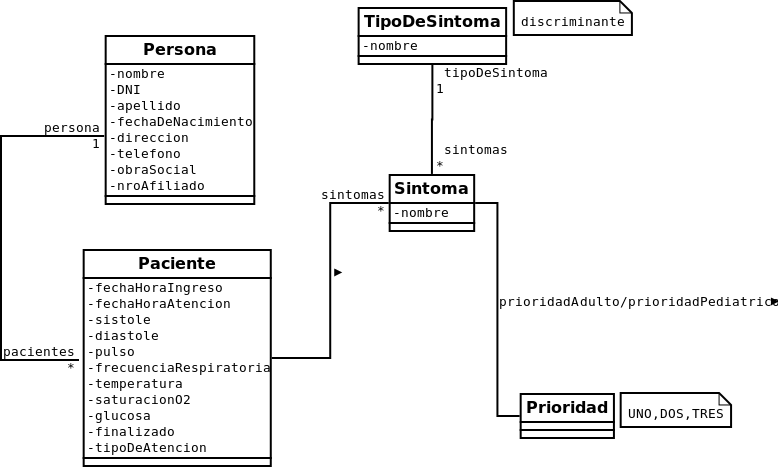
\includegraphics[width=1.2\textwidth]{triage.png}
\caption{Diagrama de clases del dominio}
\end{figure}


\subsection{Detalle técnico}
?

\subsection{Problemas que tuvimos}
?

\subsection{Detalles interesantes del código}
En el caso de que los haya 




\subsection{Testing}
Herramientas que usamos para testear, qué tipo de testing hicimos (funcional, unitario, de integración...)
\subsubsection{Funcional}
Selenium.. / Protractor / Casper
\subsubsection{Unitario}
Con Grails
\subsubsection{Integración}
Con Grails
\subsection{Deploy e Instalación}
.war
Tomcat
H2
Postgres

Cómo realizamos la instalación en el entorno de trabajo donde se usará el producto
\subsubsection{Manual de usuario}
Se confeccionó un manual de usuario...
\subsubsection{Aprendizaje del usuario}
Cuánto tiempo llevó explicar el sistema, si fue fácil de entender..